\subsection{Gépi tanulás}
\begin{frame}{Gépi tanulás}
    \begin{itemize}
        \item Egy algoritmus tanul, ha egy feladat megoldása során olyan változások következnek be a működésében, hogy később ugyanazt a feladatot jobban (eredmény, hatékonyság) képes megoldani, mint korábban
        \item Konkrét utasítások nélkül
        \item Tanító mintákra van szükség, teszt mintával ellenőrizzük az algoritmust
        \item Felügyelt, felügyelet nélküli, megerősítéses tanulás
    \end{itemize}
\end{frame}

\begin{frame}{Felügyelt tanulás}
    \begin{itemize}
        \item {\bf Tanító minta}: a minták elvárt kimenete ismert
        \item {\bf Teszt mintával} ellenőrizzük a modell általánosító képességét
        \item Két nagy csoport: osztályozás és regresszió (előrejelzés)
        \item Példák: kép és spam felismerése, időjárás-előrejelzés, népességnövekedés
    \end{itemize}
\end{frame}

\begin{frame}{Felügyelt tanulás - Várjunk-e az asztalra?}
    \centering
    \begin{tikzpicture}
        [no/.style={rectangle,draw=red!50,fill=red!20,thick},
         yes/.style={rectangle,draw=blue!50,fill=blue!20,thick},
         question/.style={rectangle,draw},
         every node/.style={node distance=7mm},
         dec/.style={midway,fill=white}]
        
        \node[no] (n1) {Nem};
        \node[yes] (y1) [right=of n1] {Igen};
        \node[question] (q1) [above=of y1] {Barátok?}
            edge [->] node[auto,swap] {\scriptsize Nincs}   (n1)
            edge [->] node[dec]      {\scriptsize Néhány}  (y1);
        
        % Várakozási idő és annak gyerekei
        \node[no]       (n2) [below=of y1] {Nem};
        \node[question] (q2) [right=of y1] {Várakozási idő?}
            edge [<-] node[dec] {\scriptsize Sok} (q1)
            edge [->] node[dec] {\scriptsize >60} (n2);
            
        \node[question] (q3) [right=of n2] {Alternatíva?}
            edge [<-] node[dec] {\scriptsize 30-60} (q2);
            
        \node[question] (q4) [right=of q3] {Éhes?}
            edge [<-] node[dec] {\scriptsize 10-30} (q2);
        
        \node[yes] (y2) [right=of q4] {Igen}
            edge [<-] node[dec] {\scriptsize 0-10} (q2);
        
        % Alternatíva és Éhes gyerekei
        \node[question] (q5) [below=of n2] {Foglalás?}
            edge [<-] node[dec] {\scriptsize Nincs} (q3);
        \node[question] (q6) [right=of q5] {P/Szo?}
            edge [<-] node[dec] {\scriptsize Van} (q3);
        \node[question] (q7) [below=of y2] {Alternatíva?}
            edge [<-] node[dec] {\scriptsize Igen} (q4);
        \node[yes] (y3) [left=of q7] {Igen}
            edge [<-] node[dec] {\scriptsize Nem} (q4);
        
        % Foglalás és P/Szo gyerekei
        \node[yes] (y4) [below=of q5] {Igen}
            edge [<-]node[dec] {\scriptsize Van} (q5);
        \node[question] (q8) [left=of y4] {Bár?}
            edge [<-] node[dec] {\scriptsize Nincs} (q5);
        \node[no] (n3) [right=of y4] {Nem}
            edge [<-] node[dec] {\scriptsize Nem} (q6);
        \node[yes] (y5) [right=of n3] {Igen}
            edge [<-] node[dec] {\scriptsize Igen} (q6);
            
        % Bár gyerekei
        \node[no] (n4) [below=of q8] {Nem}
            edge [<-] node[dec] {\scriptsize Nem} (q8);
        \node[yes] (y5) [right=of n4] {Igen}
            edge [<-] node[dec] {\scriptsize Igen} (q8);
        
        % Alternatíva gyerekei
        \node[yes] (y6) [below=of q7] {Igen}
            edge [<-] node[dec] {\scriptsize Nem} (q7);
        \node[question] (q9) [right=of y6] {Esik?}
            edge [<-] node[dec] {\scriptsize Igen} (q7);
        \node[no] (n5) [below=of y6] {Nem}
            edge [<-] node[dec] {\scriptsize Nem} (q9);
        \node[yes] (y8) [right=of n5] {Igen}
            edge [<-] node[dec] {\scriptsize Igen} (q9);
    \end{tikzpicture}
\end{frame}


\begin{frame}{Nemfelügyelt tanulás}
    \begin{itemize}
        \item Tanító minta bemenő adatokkal, nincs meg az elvárt kimenet
        \item Kérdés: van-e valami struktúra? 
        \item Példa: \href{https://news.google.com/}{Google News}
    \end{itemize}
    
    % \centering
    % \begin{tikzpicture}
    %     \node<1> (img1) {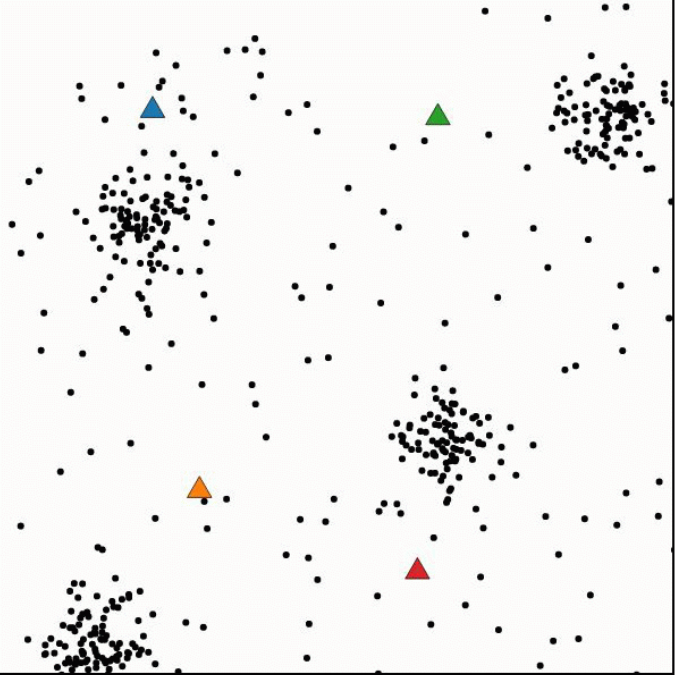
\includegraphics[scale=0.25]{figures/k-means-1.png}};
    %     \node<2> (img2) {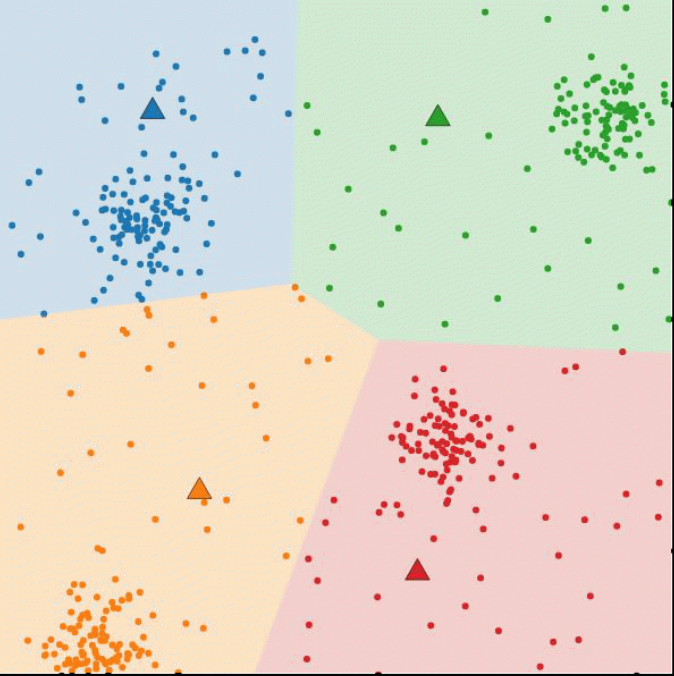
\includegraphics[scale=0.25]{figures/k-means-2.png}};
    %     \node<3> (img3) {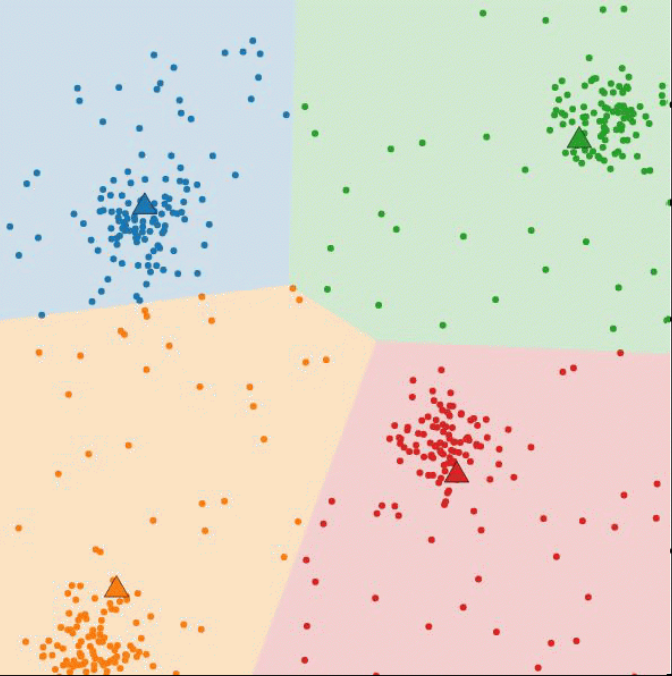
\includegraphics[scale=0.25]{figures/k-means-3.png}};
    %     \node<4> (img4) {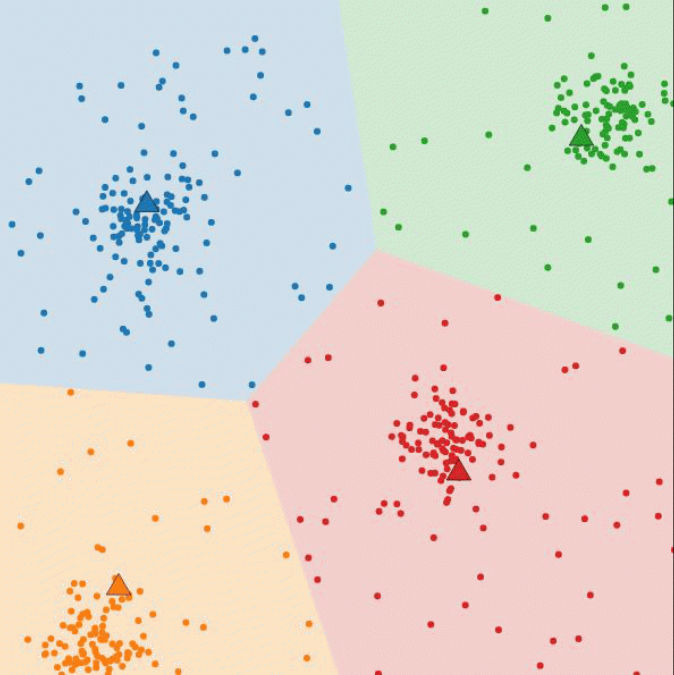
\includegraphics[scale=0.25]{figures/k-means-4.png}};
    %     \node<5> (img5) {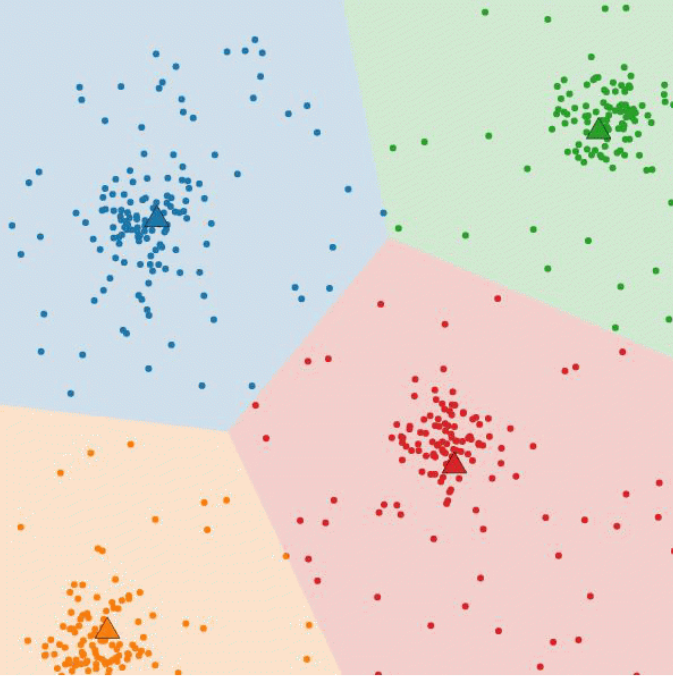
\includegraphics[scale=0.25]{figures/k-means-5.png}};
    %     \node<6> (img6) {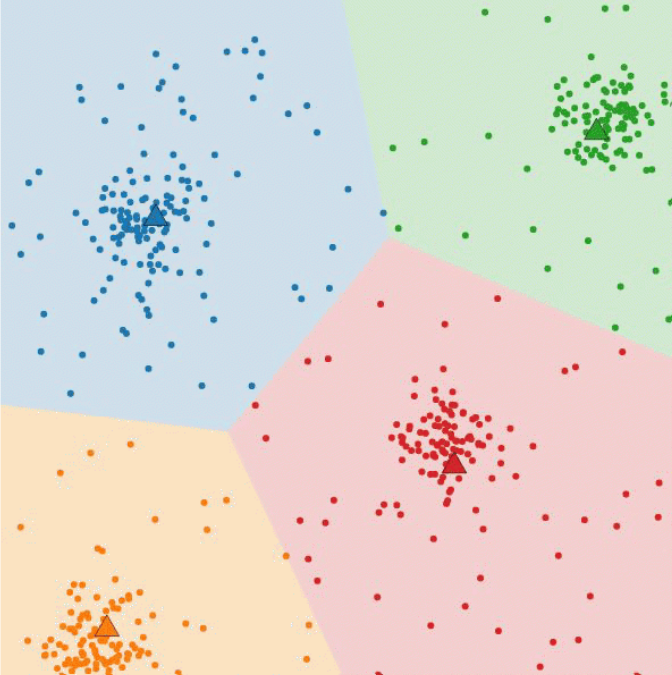
\includegraphics[scale=0.25]{figures/k-means-6.png}};
        
        % \node<7> (img7) {\includegraphics[scale=0.6]{figures/color1.png}};
        % \node<8> (img8) {\includegraphics[scale=0.6]{figures/color2.png}};
        % \node<9> (img9) {\includegraphics[scale=0.6]{figures/color3.png}};
    % \end{tikzpicture}
\end{frame}

\begin{frame}{Megerősítéses tanulás}
    \begin{itemize}
        % \item Példa: \href{https://deepmind.com/research/case-studies/alphago-the-story-so-far}{AlphaGo} (2015 október, 5-0)
        \item Példa:
        \begin{itemize}
            \item \href{https://deepmind.com/research/case-studies/alphago-the-story-so-far}{AlphaGo} (2015 október, 5-0)
            \item \href{https://www.youtube.com/watch?v=VMp6pq6_QjI}{AI Learns to Park (Youtube)}
            \item \href{https://www.youtube.com/watch?v=CqYKhbyHFtA}{Two AI Fight for the same parking spot (Youtube)}
        \end{itemize}
        \item Nincs visszajelzés, hogy mi a jó vagy rossz
        \item Az algoritmus megtanulja, hogy {\it melyik a jó lépés}
        \item Mi lehet megerősítés? Mikor kap az algoritmus megerősítést?
    \end{itemize}
\end{frame}
